\documentclass[a4paper]{article}

\usepackage{INTERSPEECH2021}

% Put the lab number of the corresponding exercise
\title{NLU course projects lab 4: LM}
\name{Nicola Muraro (248449)}

\address{University of Trento}
\email{nicola.muraro@studenti.unitn.it}

\begin{document}

\maketitle

\section{Introduction}
The purpose of this assignment is to implement a language model based on neural architectures.
Specifically, the task of this model is to predict the next token given a set of tokens, referred to as the context.
To achieve this goal, I used an LSTM on which several modifications were made to improve its performance. 
In the first part of the assignment, various optimisers were analysed alongside the use of dropout. In the second part, instead I implemented more sophisticated regularisation techniques described in the article written by Merity et al. \cite{merity2017regularizing}.
This report briefly summarises the studies conducted and the results.

\section{Implementation details}
The first part of this assignment focuses on studying LSTM as the foundation of our architecture, followed by two incremental modifications: adding dropout layers and using AdamW.
I started by replacing the original architecture (based on RNN) with LSTM to establish an initial baseline.
Next, I made the first modification by adding dropout layers: one after the embedding layer and another before the output layer.
Finally, I implemented the last required modification by replacing SGD with AdamW. Since changing the optimiser also requires adjusting the learning rate, I made the necessary adjustments to the learning rate to ensure an optimal performance.

The second part involves starting from the initial network (LSTM with SGD) and incrementally applying regularisation techniques outlined by Merity et al. \cite{merity2017regularizing}.
First, I implemented weight tying between the embedding layer and the output layer.
This technique allows multiple layers in the network to share the same weights, aiming to regularise the entire architecture.
To enable weight sharing, the layers involved must have the same dimensions, so I adjusted their sizes to ensure compatibility.
The second modification involved using Variational Dropout, a technique that applies the same dropout mask.
In practice, this means reusing the same dropout mask instead of sampling a new one at each model call.
With this setup, the mask can be changed once per epoch and/or differ between layers.
During my tests, I experimented with both approaches to determine the most effective configuration.
Finally, I implemented the last modification: using Non-monotonically Triggered AvSGD. This is a variant of AvSGD where the switch to AvSGD is based on the network’s state during training.
Specifically, if SGD fails to improve the solution over several consecutive epochs, it is replaced with AvSGD in the hope of further optimizing the solution.
Since the timing of this switch is not predetermined, this technique is expected to provide additional performance improvements compared to both standard SGD and AvSGD.

\section{Results}
The results used to evaluate the effectiveness of the implemented techniques were obtained using the evaluation set. This approach ensures better generalisation. Using the evaluation set to fine-tune hyper-parameters and find an optimal configuration allows for more reliable results on the test set.
In general, the best machine learning models have high capacity and are properly regularised. Since many of the previously applied techniques are forms of regularisation, I started with a relatively large model.
For all configurations, the batch size for the training segment was kept constant at 64, while for the evaluation it was set at 128.


In the first part, the initial model was created with the following specifications: \(emb \textunderscore size=600, hidden \textunderscore size=500, lr=1.5\).
The use of dropout yielded better results with a probability of \(p=0.3\). Finally, after replacing the optimizer with AdamW, I adjusted the learning rate to 0.0005.
As we can see from the results shown in table \ref{tab:results1}, only the first two modifications led to improved performance. 
We can observe that the addition of AdamW does not result in an improvement in performance on the validation set. However, it leads to an improvement on the test set. This might suggest better generalization by this optimizer, but not consistently across both datasets. Consequently, as it does not improve the values on the validation set, this modification was disregarded in the final model. For optimal generalization we cannot implement a modification based solely on its performance on the test set, since we generally would not have access to such data.
The training process of the best model is depicted in Figure \ref{fig:fig1}.

\begin{table}[h]
  \centering
  \begin{tabular}{|c|c|c|}
    \hline
    \textbf{Model} & \textbf{Eval PPL} & \textbf{Test PPL} \\
    \hline
    LSTM & 144.09 & 139.51 \\
    LSTM with dropout & 115.45 & 111.07 \\
    LSTM with dropout, AdamW & 119.01 & 109.17\\
    \hline
  \end{tabular}
  \caption{Perplexity values for the first part of the assignment}
  \label{tab:results1}

\end{table}

\begin{figure}[h]
  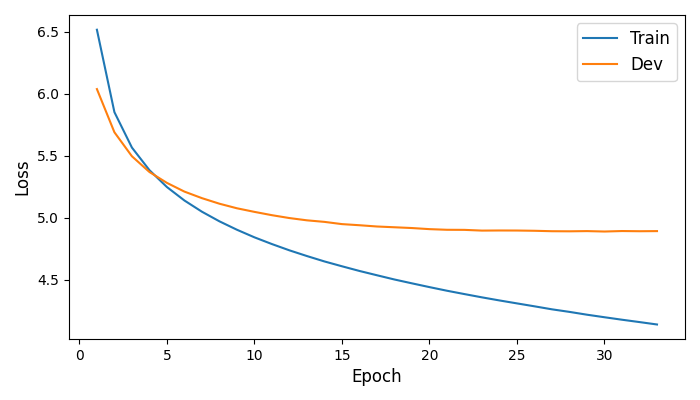
\includegraphics[width=\linewidth]{./images/plot_1_loss.png}
  \caption{Trainig loss for the best model of the first part}
  \label{fig:fig1}
\end{figure}


For the second part, starting with the same configuration as before \((emb \textunderscore size=600, hidden \textunderscore size=500, lr=1.5)\), I modified the layer sizes to use weight tying.
The model now has \(emb \textunderscore size=hid \textunderscore size=600\).
Regarding Variational Dropout, I tested all four possible combinations for changing the mask: (1) one mask for both layers (fixed); (2) one mask for both layers (changed every epoch); (3) two masks (one per layer, fixed); (4) two masks (one per layer, changed every epoch). The best performance was achieved with the third option: using a different mask for each layer of dropout and changing it every epoch.
Finally, as shown in table \ref{tab:results2}, I completed the assignment using NT-AvSGD.
The last model switches to AvSGD only in the last few epochs, yet this still enables the model to reach a lower perplexity value.
In Figure \ref{fig:fig2}, the model's training progression is represented.

\begin{table}[h]
  \centering
  \begin{tabular}{|c|c|c|}
    \hline
    \textbf{Tecnique} & \textbf{Eval PPL} & \textbf{Test PPL} \\
    \hline
    W.Tying & 130.78 & 128.35 \\
    W.Tying, Var.Drop. & 129.43 & 125.85 \\
    W.Tying, Var.Drop., NT-AvSGD & 124.56 & 122.22 \\
    \hline
  \end{tabular}
  \caption{Perplexity values for the second part of the assignment}
  \label{tab:results2}

\end{table}

\begin{figure}[h]
  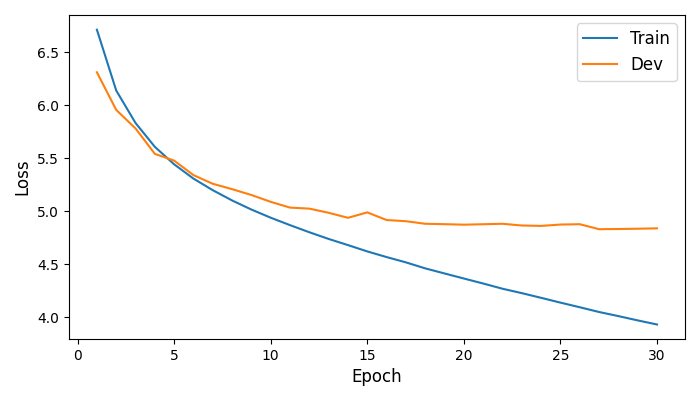
\includegraphics[width=\linewidth]{./images/plot_2_loss.png}
  \caption{Trainig loss for the best model of the second part}
  \label{fig:fig2}
\end{figure}


\bibliographystyle{IEEEtran}

\bibliography{mybib}


\end{document}
